\documentclass[format=sigconf,review=true]{acmart}
\usepackage{tikz}
\usetikzlibrary{matrix}
\usepackage{listings}
\title{Verifying file systems with ACL2}
\subtitle{Towards verifying data recovery tools}
\author{Mihir P. Mehta}

\affiliation{%
  \institution{University of Texas at Austin}
  \city{Austin}
  \state{TX}
  \country{USA}}
\email{mihir@cs.utexas.edu}

\thanks{This work is supported by a grant from the NSF. }

\begin{document}
\lstset{language=Lisp}

\maketitle

\section{Introduction}

In this paper, we describe work in progress to model and verify
filesystems using the ACL2 theorem prover.

\section{Motivation}
Filesystems are ubiquitous, and a critical factor in the security and
performance of all applications. Yet, they remain poorly understood,
a problem which has been exacerbated by the complexity of modern
filesystems which use redundancy and caching in order to be faster and
more reliable. As a consequence, many tools which interact deeply with
the filesystem, such as file deletion and file recovery tools, have
become more vulnerable to bugs because of the complexity of these
tasks. Thus, it is worthwhile to work towards formally verifying the
guarantees provided by a filesystem.

\section{Modelling a filesystem}

In order to make our proofs of correctness tractable, we choose to
make several verified filesystem models in increasing order of
complexity. This approach supports incremental proof strategies,
providing us with a choice between proving a model equivalent to the
next, and simply adapting existing proofs for the next model.

While starting out, we faced a decision about the file system
operations we should provide. We decided against implementing the
entirety of the Linux VFS interface\cite{johnson_1996}, reasoning that this would require
us to implement 19 inode operations, 6 dentry operations and 22 file
operations. Following the  example of the Google File System
\cite{ghemawat2003google}, we decided to restrict ourselves to a small
number of fundamental file system operations - namely reading, writing,
creating, and deleting a file. This excludes the operations of opening
and closing a file; we hope to implement these when they become
necessary for verification in a multiprogramming environment.

\section{Model 1}
The intuitive mental model of a filesystem is a tree, which remains
useful even though it fails for filesystems with links. Accordingly,
it is appropriate for our first model, which will serve as a
specification for all later models, to be a literal tree. Our
filesystem recogniser, \texttt{l1-fs-p}, recognises
\texttt{symbol-alist}s where each cdr of a pair in the alist satisfies
either \texttt{stringp} (denoting a regular file) or \texttt{l1-fs-p}
(denoting a subdirectory).

Below, we include a sample of a filesystem tree that is recognised by
l1-fs-p, and a code listing.

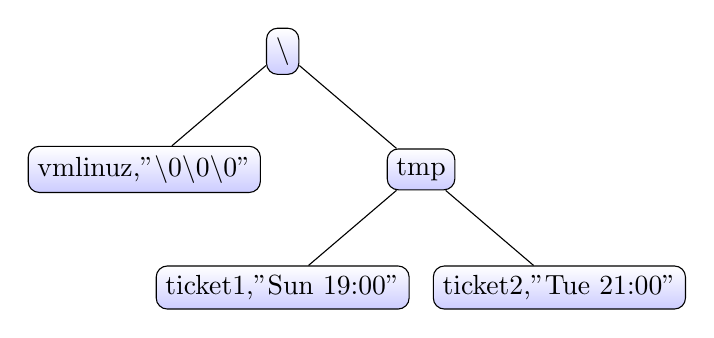
\begin{tikzpicture}[sibling distance=10em,
  every node/.style = {shape=rectangle, rounded corners,
    draw, align=center,
    top color=white, bottom color=blue!20}]]
  \node {\textbackslash}
    child { node {vmlinuz,{"}\textbackslash0\textbackslash0\textbackslash0{"}} }
    child { node {tmp}
      child { node {ticket1,{"}Sun 19:00{"}}}
      child { node {ticket2,{"}Tue 21:00{"}}}};
\end{tikzpicture}

\begin{lstlisting}
(DEFUN
  L1-FS-P (FS)
  (DECLARE (XARGS :GUARD T))
  (IF
   (ATOM FS)
   (NULL FS)
   (AND
    (LET ((DIRECTORY-OR-FILE-ENTRY (CAR FS)))
         (IF (ATOM DIRECTORY-OR-FILE-ENTRY)
             NIL
             (LET
              ((NAME (CAR DIRECTORY-OR-FILE-ENTRY))
               (ENTRY (CDR DIRECTORY-OR-FILE-ENTRY)))
              (AND (SYMBOLP NAME)
                   (OR (STRINGP ENTRY)
                       (L1-FS-P ENTRY))))))
    (L1-FS-P (CDR FS)))))
\end{lstlisting}

\section{Model 2}
Model 1 can hold unbounded text files and nested directory
structures. However, real filesystems include metadata, and including
metadata in our filesystem representation also allows us to define a
notion of "consistency" wherein the actual contents of a regular or
directory file are checked for agreement with the metadata. Thus, in
our next model, we add an extra field for length of a
regular file. We also create a simple version of fsck that checks
file contents for consistency with the stated length, and verify
that the operations for writing, creating and deleting preserve this
notion of consistency.

Below, we include a sample of a filesystem tree that is recognised by
l2-fs-p, and a code listing.

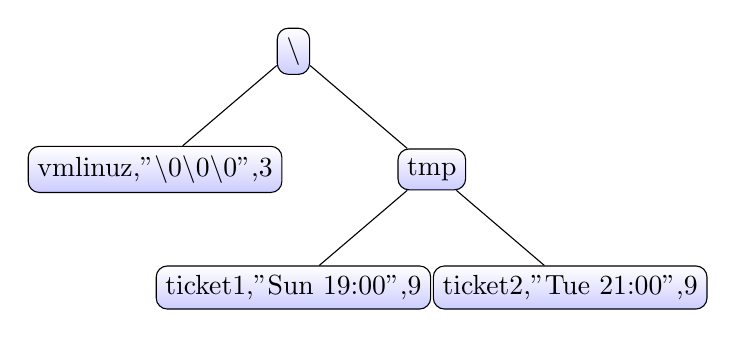
\begin{tikzpicture}[sibling distance=10em,
  every node/.style = {shape=rectangle, rounded corners,
    draw, align=center,
    top color=white, bottom color=blue!20}]]
  \node {\textbackslash}
    child { node {vmlinuz,{"}\textbackslash0\textbackslash0\textbackslash0{"},3} }
    child { node {tmp}
      child { node {ticket1,{"}Sun 19:00{"},9}}
      child { node {ticket2,{"}Tue 21:00{"},9}}};
\end{tikzpicture}

\begin{lstlisting}
(DEFUN
  L2-FS-P (FS)
  (DECLARE (XARGS :GUARD T))
  (IF
   (ATOM FS)
   (NULL FS)
   (AND
    (LET
     ((DIRECTORY-OR-FILE-ENTRY (CAR FS)))
     (IF (ATOM DIRECTORY-OR-FILE-ENTRY)
         NIL
         (LET
          ((NAME (CAR DIRECTORY-OR-FILE-ENTRY))
           (ENTRY (CDR DIRECTORY-OR-FILE-ENTRY)))
          (AND (SYMBOLP NAME)
               (OR (AND (CONSP ENTRY)
                        (STRINGP (CAR ENTRY))
                        (NATP (CDR ENTRY)))
                   (L2-FS-P ENTRY))))))
        (L2-FS-P (CDR FS)))))
\end{lstlisting}

\section{Model 3}
Next, we would like to move towards a more realistic file storage
paradigm where the contents of a regular file are broken into
fixed-size blocks and stored in an external table, which we will refer
to as the disk. In this model, we store the text of a regular file in
the disk, and retain only the indices of the relevant blocks in the
filesystem tree. For now, we consider the disk to be unbounded and
make no attempt at garbage collection. Thus, file creation and writing
operations can be represented as append operations, where the new
blocks representing the new contents of a file are simply placed at
the end of the disk with no effort to free the old blocks or erase
their contents. Similarly, deleting a file does not require any disk
operations; the blocks of such a file remain in the disk but are no longer
referred to.

As before, we include a sample of a filesystem tree that is recognised by
l3-fs-p and a code listing.

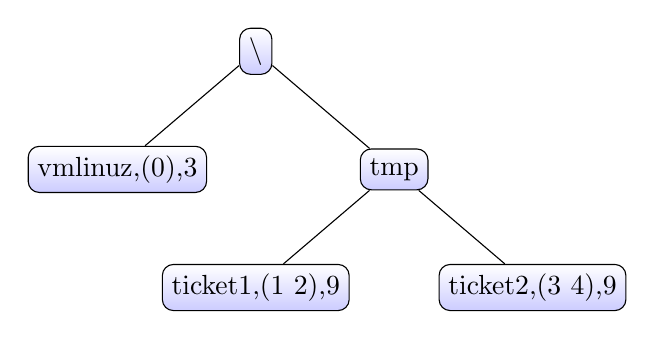
\begin{tikzpicture}[sibling distance=10em,
  every node/.style = {shape=rectangle, rounded corners,
    draw, align=center,
    top color=white, bottom color=blue!20}]]
  \node {\textbackslash}
    child { node {vmlinuz,(0),3} }
    child { node {tmp}
      child { node {ticket1,(1 2),9}}
      child { node {ticket2,(3 4),9}}};
\end{tikzpicture}

\begin{lstlisting}
(DEFUN L3-REGULAR-FILE-ENTRY-P (ENTRY)
  (DECLARE (XARGS :GUARD T))
  (AND (CONSP ENTRY)
       (NAT-LISTP (CAR ENTRY))
       (NATP (CDR ENTRY))
       (FEASIBLE-FILE-LENGTH-P (LEN (CAR ENTRY))
                               (CDR ENTRY))))

(DEFUN
  L3-FS-P (FS)
  (DECLARE (XARGS :GUARD T))
  (IF
   (ATOM FS)
   (NULL FS)
   (AND
    (LET
     ((DIRECTORY-OR-FILE-ENTRY (CAR FS)))
     (IF (ATOM DIRECTORY-OR-FILE-ENTRY)
         NIL
         (LET
          ((NAME (CAR DIRECTORY-OR-FILE-ENTRY))
           (ENTRY (CDR DIRECTORY-OR-FILE-ENTRY)))
          (AND (SYMBOLP NAME)
               (OR (L3-REGULAR-FILE-ENTRY-P ENTRY)
                   (L3-FS-P ENTRY))))))
    (L3-FS-P (CDR FS)))))
\end{lstlisting}

\section{Model 4}
In this model, we finitise our disk; this necessitates garbage
collection which we approximate through reference
counting. Since we allow neither symbolic links nor hard links in our
filesystem, the reference count of any block in the disk is either 0
or 1. This allows us to implement reference counting through an
allocation vector, i.e. an array of booleans with the same length as
the disk. Thus, in every write or delete operation, the allocation
vector entries corresponding to blocks which are no longer used must
be marked free; similarly, in every write or create operation, the
allocation vector must be scanned to find the appropriate number of
free blocks. The lockstep updates described here allow us to prove
that aliasing between different files does not occur.

The recogniser l4-fs-p is defined to be the same as l3-fs-p, which
makes our equivalence proofs simpler. This arises from the fact that
reference counting does not require any changes in the filesystem tree
or the disk. A sample filesystem tree follows, with the corresponding
disk and allocation in table \ref{model4-disk-alv}.

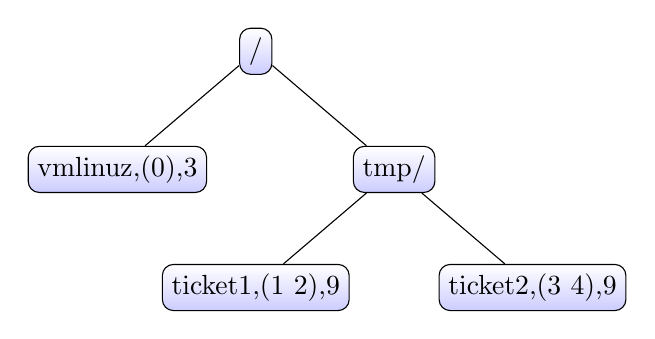
\begin{tikzpicture}[sibling distance=10em,
    every node/.style = {shape=rectangle, rounded corners,
      draw, align=center,
      top color=white, bottom color=blue!20}]]
    \node {/}
    child { node {vmlinuz,(0),3} }
    child { node {tmp/}
      child { node {ticket1,(1 2),9}}
      child { node {ticket2,(3 4),9}}};
\end{tikzpicture}
\begin{table}[]
  \centering
  \caption{Model 4 - disk and allocation vector}
  \label{model4-disk-alv}
  \begin{tabular}{|l|l|l|}
    \hline
    0 & \textbackslash0\textbackslash0\textbackslash0   & true\\ \hline
    1 & Sun 19:0 & true\\ \hline
    2 & 0        & true\\ \hline
    3 & Tue 21:0 & true\\ \hline
    4 & 0        & true\\ \hline
    5 &          & false\\ \hline
  \end{tabular}
\end{table}

An interesting insight from the proofs of correctness for model 4 was
that there is no simple transformation from instances of model 4 to
instances of model 3. The contents of a single file are always
contiguous in model 3 but not in model 4, and this makes it difficult
to derive a transformation that will support a read-over-write
proof. Thus, we chose a different strategy: defining a transformation
l4-to-l2-fs from instances of l4 to instances of model 2. Thanks to
the common definition of l4-fs-p and l3-fs-p, we were able to reuse
the already defined l3-to-l2-fs here, which again simplified our proof
effort.

\section{Model 5}
This model extends model 4 with the addition of a new kind of
metadata, namely file permissions. Incorporating read/write permissions
for the user and others, this model develops the necessary
infrastructure for more complex permissions checking mechanisms,
including user groups and access control lists. We opted to keep the
block allocation and garbage collection algorithms the same; this made
it easier to prove an equivalence between model 5 and model 4, and in
turn, the read-over-write theorems.

No new data structures are added to this model - only metadata for
file permissions and ownership. However, this is the first model for
which we added getter and setter functions for the data and metadata
in a regular file, allowing us to keep the recogniser for a regular
file disabled and simplify our proof effort.

Below, we provide a code listing for l5-fs-p and
l5-regular-file-entry-p.

\begin{lstlisting}
(DEFUND L5-REGULAR-FILE-ENTRY-P (ENTRY)
  (DECLARE (XARGS :GUARD T))
  (AND (EQUAL (LEN ENTRY) 6)
       (NAT-LISTP (CAR ENTRY))
       (NATP (CADR ENTRY))
       (FEASIBLE-FILE-LENGTH-P (LEN (CAR ENTRY)) (CADR ENTRY))
       (BOOLEANP (CAR (CDDR ENTRY)))
       (BOOLEANP (CADR (CDDR ENTRY)))
       (BOOLEANP (CAR (CDDR (CDDR ENTRY))))
       (BOOLEANP (CADR (CDDR (CDDR ENTRY))))
       (NATP (CDDR (CDDR (CDDR ENTRY))))))

(DEFUN L5-FS-P (FS)
  (DECLARE (XARGS :GUARD T))
  (IF (ATOM FS)
      (NULL FS)
    (AND (LET ((DIRECTORY-OR-FILE-ENTRY (CAR FS)))
           (IF (ATOM DIRECTORY-OR-FILE-ENTRY)
               NIL
             (LET ((NAME (CAR DIRECTORY-OR-FILE-ENTRY))
                   (ENTRY (CDR DIRECTORY-OR-FILE-ENTRY)))
               (AND (SYMBOLP NAME)
                    (OR (L5-REGULAR-FILE-ENTRY-P ENTRY)
                        (L5-FS-P ENTRY))))))
         (L5-FS-P (CDR FS)))))
\end{lstlisting}

\section {Proof approach}

Initially, we would like to prove two well-known properties from the
first-order theory of arrays, adapted to the filesystem context. These
are the well-known read-over-write properties, which show the
integrity of the filesystem.

\begin {enumerate}
\item Reading from a location after writing to the same location
  should yield the data that was written.
\item Reading from a location after writing to a different
  location should yield the same result as reading before the write.
\end {enumerate}

While these properties are simple enough to state, proving them turns
out to be surprisingly subtle. As a point of reference, proving these
properties for l1, our initial model, required us to manually specify
an induction scheme with 6 conditional branches. As noted
before, we have modelled our filesystem incrementally in order to make
our proofs tractable, thus, in each successive model, we prove a
theorem showing the model to be equivalent to the previous one. For
instance, we define the following function for transforming
instances of model 2 to model 1.

\begin{lstlisting}
(DEFUN L2-TO-L1-FS (FS)
  (DECLARE (XARGS :GUARD (L2-FS-P FS)))
  (IF (ATOM FS)
      FS
      (CONS
       (LET*
        ((DIRECTORY-OR-FILE-ENTRY (CAR FS))
         (NAME (CAR DIRECTORY-OR-FILE-ENTRY))
         (ENTRY (CDR DIRECTORY-OR-FILE-ENTRY)))
        (CONS NAME
              (IF (AND (CONSP ENTRY)
                       (STRINGP (CAR ENTRY)))
                  (CAR ENTRY)
                  (L2-TO-L1-FS ENTRY))))
       (L2-TO-L1-FS (CDR FS)))))
\end{lstlisting}

Then, we can prove the implementation of the write operation in model
2 correct with respect to the specification of model 1 by proving the
property illustrated below.

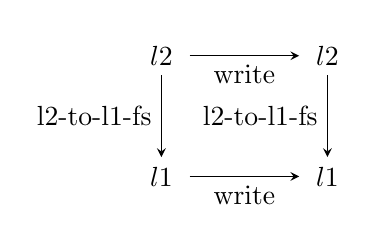
\begin{tikzpicture}
  \matrix (m) [matrix of math nodes,row sep=3em,column sep=4em,minimum width=2em]
  {
     l2 & l2 \\
     l1 & l1 \\};
  \path[-stealth]
    (m-1-1) edge node [left] {l2-to-l1-fs} (m-2-1)
            edge node [below] {write} (m-1-2)
    (m-2-1.east|-m-2-2) edge node [below] {write} (m-2-2)
    (m-1-2) edge node [left] {l2-to-l1-fs} (m-2-2);
\end{tikzpicture}

Similarly, we can prove the implementation of the read operation in
model 2 correct with respect to the spec in model 1.

\begin{tikzpicture}
  \matrix (m) [matrix of math nodes,row sep=3em,column sep=4em,minimum width=2em]
  {
     l2 & text \\
     l1 \\};
  \path[-stealth]
    (m-1-1) edge node [left] {l2-to-l1-fs} (m-2-1)
            edge node [below] {read} (m-1-2)
    (m-2-1.east|-m-2-2) edge node [below] {read} (m-1-2);
\end{tikzpicture}

Combining these proofs as shown below, we are able to prove the read-after-write
properties for model 2 based on our proof for model 1.

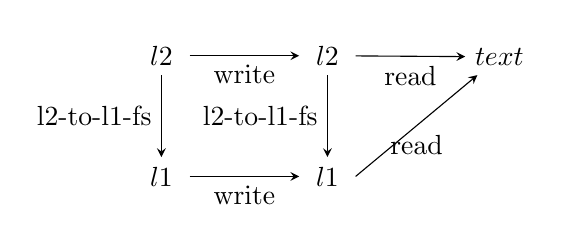
\begin{tikzpicture}
  \matrix (m) [matrix of math nodes,row sep=3em,column sep=4em,minimum width=2em]
  {
     l2 & l2 & text \\
     l1 & l1 \\};
  \path[-stealth]
    (m-1-1) edge node [left] {l2-to-l1-fs} (m-2-1)
            edge node [below] {write} (m-1-2)
    (m-2-1.east|-m-2-2) edge node [below] {write} (m-2-2)
    (m-1-2) edge node [left] {l2-to-l1-fs} (m-2-2)
            edge node [below] {read} (m-1-3)
    (m-2-2.east) edge node [below] {read} (m-1-3);
\end{tikzpicture}

\section{Evaluation}
At present, the codebase spans 6017 lines of ACL2 code, including 118
function definitions and 419 defthm events. Some of this data was
obtained by David A. Wheeler's sloccount tool.

In table \ref{certification-timing-table} we note the time taken to certify
the models in ACL2, as well as some infrastructure upon which the
models are built.

Additionally, for model 5, we ran some tests involving writing a
string to a file in the filesystem. The results are shown in table
\ref{write-timing-table}.

\begin{table}[]
  \centering
  \caption{Time taken to prove models}
  \label{certification-timing-table}
  \begin{tabular}{ll}
    Model 1 & 1.167s \\
    Model 2 & 5.672s \\
    Model 3 & 7.628s \\
    Model 4 & 31.045s \\
    Model 5 & 19.925s \\
    Miscellaneous shared lemmas & 2.577s \\
  \end{tabular}
\end{table}

\begin{table}[]
\centering
\caption{Time taken to write strings}
\label{write-timing-table}
\begin{tabular}{ll}
Length of string    & Time taken  \\
4096    & 0.05s  \\
16384   & 0.10s  \\
65536   & 0.34s  \\
262144  & 1.55s  \\
1048576 & 10.75s
\end{tabular}
\end{table}

\section{Future work}
Having incorporated garbage collection and metadata into the
filesystem model, the next challenge is the linearisation of the
filesystem model. This would be more in keeping
with realistic file systems that do not require an in-memory tree
representation, but still allow tree traversal through systematic
lookups in the disk.

We are also planning to add the system calls open and close with the
introduction of file descriptors. This would be a step towards the
study of concurrent FS operations. An alternative approach would be to
model concurrent operations after the fashion of Sun NFS
\cite{sandberg1985design}; this is also under consideration.

Eventually, we would like to emulate the FAT32 filesystem. This would
be a step towards verified versions of fsck and file recovery tools,
which would be based on our proofs about the underlying filesystem.

\section{Related work}
Fileystem verification is a research topic of long standing. An early
effort is \cite{}, where the authors opted to use an interactive
theorem prover (Athena) to prove a simulation relation between their
implementation and a specification of their own creation.

A landmark paper in the kernel verification space is \cite{}. The authors,
here, took a microkernel approach, and as a consequence filesystem
operations do not appear in the kernel they verified. They did, later,
take up the problem in \cite{}.

Currently, the state of the art is represented by Haogang
Chen's dissertation work \cite{DBLP:conf/usenix/ChenZCCKZ16}, in which
the author uses Coq to build a filesystem (named FSCQ) which is proven
safe against crashes. This implementation was exported into Haskell,
and showed comparable performance to ext4 when run on the Linux kernel
through the FUSE layer.

Another recent work in this space, Hyperkernel
\cite{Nelson:2017:HPV:3132747.3132748} is a "push-button" kernel verification
effort using the Z3 SMT solver. However, in order to accommodate the
limitations of Z3, Hyperkernel approximates by changing POSIX system
calls for ease of verification.

Our work takes a different approach - our aim is to produce verified
models of existing filesystems that have binary compatibility with the
filesystem layout read and written by the corresponding
implementation. This allows us to find bugs in existing filesystems,
which is not addressed by Chen's work.

\section{Conclusion}
Through this work, we have gone into some depth on an approach towards
implementing a filesystem with several essential features (block
allocation, file-level metadata, garbage collection) found in real
filesystems. In the process, we have demonstrated ACL2's capability to
deal with systems-level problems in addition to the hardware
verification problems to which it has traditionally been applied.

\section{Obtaining the code}
This work is hosted on GitHub, under the GPL 3.0 licence. The code
repository can be cloned anonymously using the HTTPS URL
https://github.com/airbornemihir/turbo-octo-sniffle.git, and the
repository itself can be viewed at
https://github.com/airbornemihir/turbo-octo-sniffle.

\bibliographystyle{ACM-Reference-Format}
\bibliography{references}

\end{document}
